\section{Methodology Description}
\label{S:t4}
Pedestrian movement patterns are highly correlated both temporally and spatially \cite{song2016deeptransport}. Recurrent Neural Networks (RNNs) are a popular choice to deal with the problem by treating mobility patterns of a pedestrian as a sequence prediction problem. However, it has been shown that RNNs are not capable of remembering long-term temporal and spatial dependencies as a result of the problem of vanishing gradient~\cite{hochreiter1997long}. Introduced in \cite{hochreiter1997long}, Long Short-Term Memory (LSTM) is a modification to traditional RNN architecture that enables learning sequence labels for longer time intervals by implementing four interactive gates. In \cref{fig:LSTM}, a schematic representation of a typical LSTM network is depicted. To compute a sequence of output units \(Y=(y_1,y_2,...,y_T)\), from a sequence of inputs \(X=(X_1,X_2,...X_T)\), the following equations should be followed iteratively over time \textit{t}:

\begin{itemize}
    \item forget gate: 
    \begin{equation}
        f_t=\sigma(W_fx_t+U_fh_{t-1}+b_f))
    \end{equation}
    \item input gate:
    \begin{equation}
    i_t=\sigma(W_ix_t+U_ih_{t-1}+b_i)
    \end{equation}
    \item Cell state:
    \begin{equation}
    c_t=f_t\odot c_{t-1}+i_t\odot \sigma(W_cx_t+U_ch_{t-1}+b_c) 
    \end{equation}
    \item output gate:
    \begin{equation}
    o_t=\sigma(W_ox_t+U_oh_{t-1}+b_o)
    \end{equation}
    \item hidden state:
    \begin{equation}
    h_t=o_t\odot \sigma(c_t)
    \end{equation}
    \item output layer:
    \begin{equation}
    y_t=\sigma(W_{y}h_t+b_y
    \end{equation}
\end{itemize}
in which: \(f_t,i_t,o_t\) are the activation vectors of forget gate, input gate and output gate respectively. \(h_t\) is the hidden state vector, which plays the role of an output vector of LSTM unit, \(c_t\) is the cell state vector, \(W,U\) and \(b\) are the weights and biases to be learned in the training phase, and \(\odot\) represents the element-wise product. \(\sigma\) represents the activation functions on respective layers. 
\begin{figure}
    \centering
    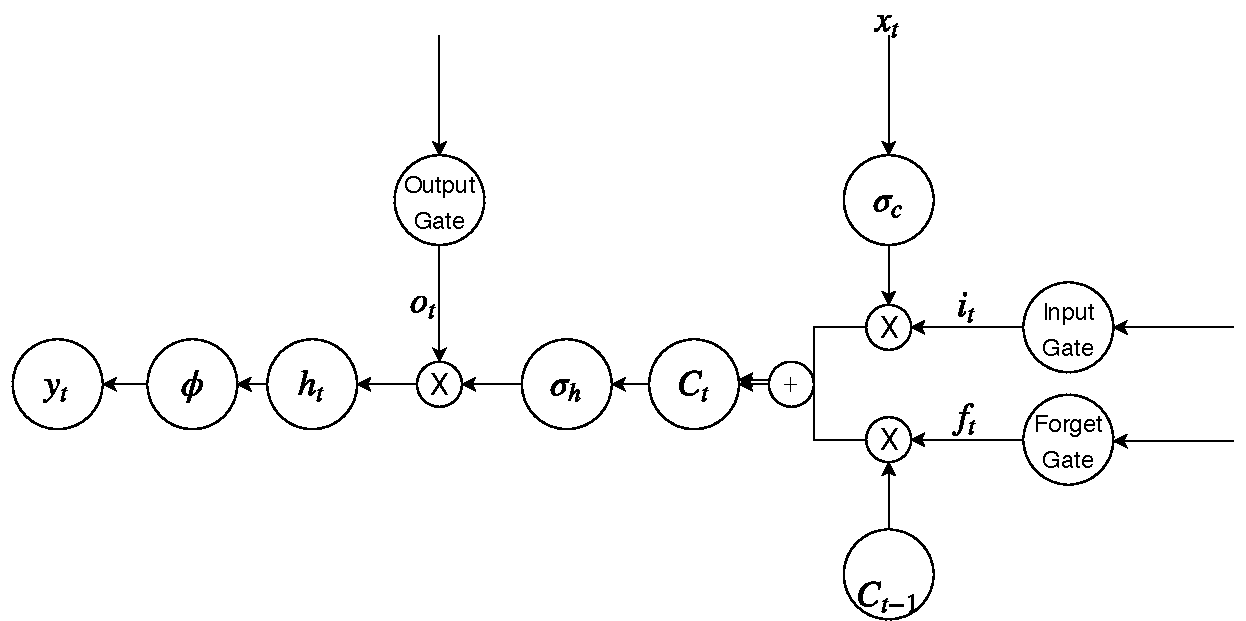
\includegraphics[scale=0.6]{chapter_6/figures/lstm.pdf}
    \caption{Schematic framework of an LSTM block}
    \label{fig:LSTM}
\end{figure}

In this study, we propose, \textit{Aux-LSTM}, a novel framework consisting of multi-input LSTM layers and fully connected dense layers, to predict the next coordinates of pedestrians as output. Initial steps of time-series data, i.e., coordinates, head orientations, and distance to vehicle, are used as input to the LSTM layers. The output of the LSTM layers will then merge with extra information from environmental variables, and the mergers enter a series of fully connected dense layers to predict the trajectory of the pedestrians in the rest of their crossing. Input time-series data are defined in two ways: time-based and distance-based. In the time-based approach, the coordinates of the pedestrian in the next $t_2$ seconds are predicted based on their last $t_1$ seconds of behaviours. At each point during the cross, pedestrian coordinates, head orientations, and their distance to the approaching vehicle during the last $t_1$ seconds are used as time-series input to predict the coordinates of the pedestrian in the next $t_2$ seconds. In the distance-based type of models, however, the proportion of data that is used as input, $p$, is defined as the proportion of lane width that the pedestrian has passed when the algorithm tries to predict the coordinates of the pedestrian in the rest of the cross. For instance, if $p$ is set to 0.3, the framework tries to predict the trajectory of the pedestrians based on their trajectory in the first 30\% of the lane width. Different values of $t_1$, $t_2$ and $p$ are tested in order to provide insights into the required method of data preparation.

As a regularization mechanism to the framework, the model is supervised through two identical loss functions. Both loss functions are defined as the euclidean distance between predicted and actual coordinates. By using the loss function after the LSTM layers, a.k.a. secondary loss, we allow smoother training for the framework. Batch Normalization and Dropout layers are also used in order to reduce overfitting in the model. \cref{fig:Tframe} depicts the general framework of Aux-LSTM.
\begin{figure}
    \centering
    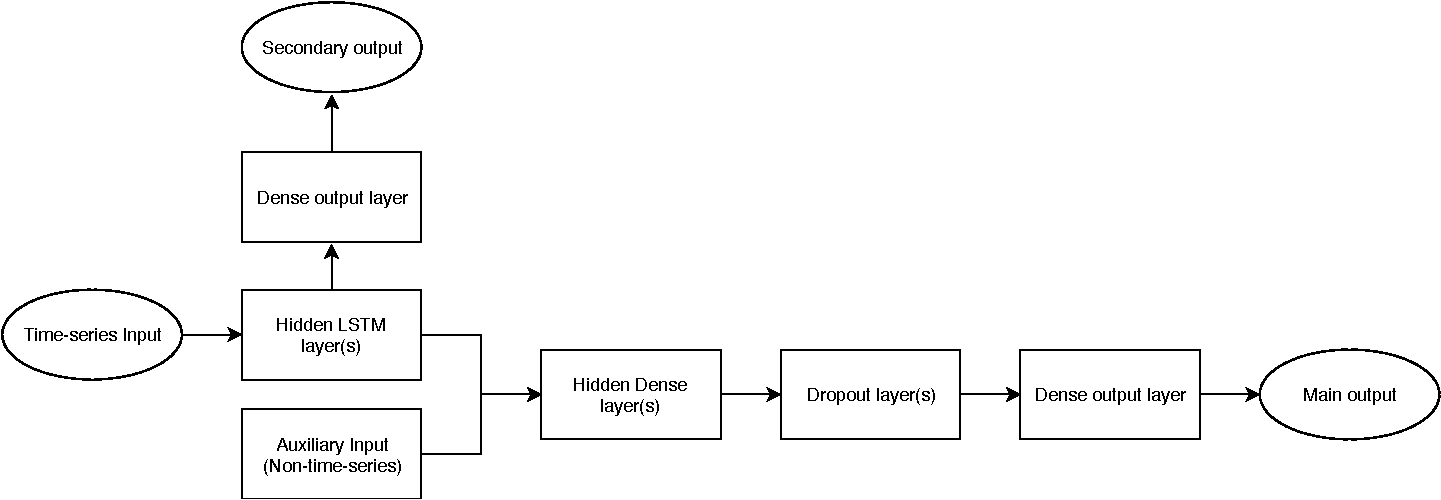
\includegraphics[scale=0.57]{chapter_6/figures/frame.pdf}
    \caption{Schematic framework of Aux-LSTM}
    \label{fig:Tframe}
\end{figure}